\chapter{Inverse Functions}
%\addcontentsline{toc}{chapter}{1 Graphs}
%%%%%%%%%%%%%%% SECTION HEADER %%%%%%%%%%%%%%%%
\rhead{7}
\lhead{Inverse Functions}
%%%%%%%%%%%%%%%%%%% START %%%$%%%%%%%%%%%%%%%%%
\section{Inverse functions}
When a value goes into a function it is called the input. The result that we get
when we evaluate the function is called the output. Figure \ref{fig:funct} shows the function $f$, where an octahedron, representing input, enters through the function machine's input funnel, and the function machine spits out a particular sphere, representing output.\\
When working with functions
sometimes we will know the output and be interested in what input gave us the
output. To model this behavior, we use an inverse function. As the name suggests an inverse
function undoes whatever the function did. If a function is named $f(x)$, the
inverse function will be named $f^{−1}(x)$ (read “$f$ inverse of $x$”). Figure \ref{fig:funct_inv} illustrates the inverse of $f$. The  inverse works backward meaning if the input is a sphere, it will return an octahedron--undoing $f$.
%
\begin{figure}[ht]
    \centering
    \subfloat[Function $f(x)$]
    {
    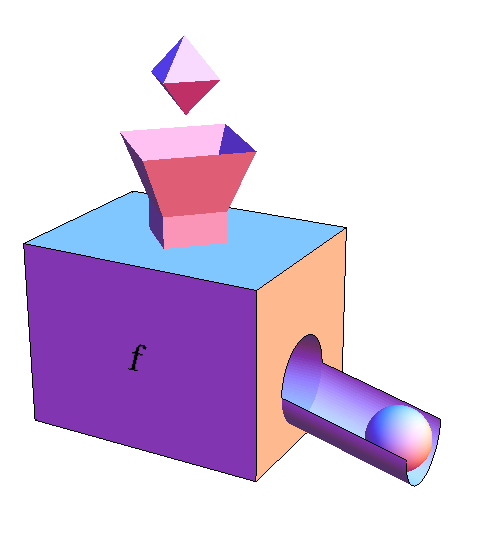
\includegraphics[width=5cm]{Pics/function_machine_f.png}
    \label{fig:funct}
    }%
    \qquad
    \subfloat[Inverse function $f^{-1}(x)$]
    {
    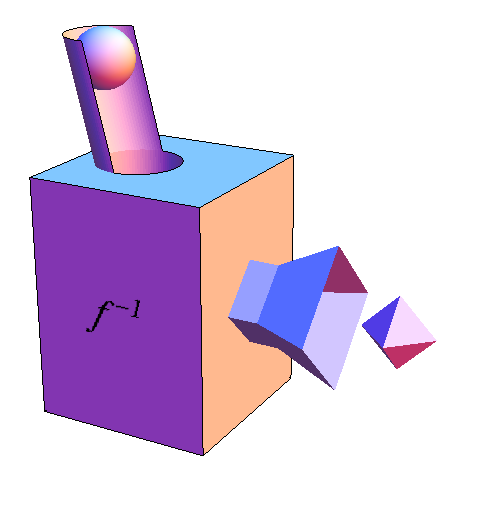
\includegraphics[width=5cm]{Pics/function_machine_finv.png}
    \label{fig:funct_inv}
    }%
    \caption{Function, $f(x)$, and its inverse, $f^{-1}(x)$, as machines.}%
    \label{fig:funct_vs_inv}%
\end{figure}
%
\begin{nt}
$f^{-1}(x) \neq \frac{1}{f(x)}$. It is very important not to confuse function notation with negative exponents. But only a symbol to let us know that this function is the inverse of $f$.
\end{nt}
%
\begin{tcolorbox}[
                    title=Domain and range of inverse function,
                    fonttitle=\bfseries,
                    colframe=blue!70!red,
                    colback=white]
    \begin{itemize}
        \item The domain of $f^{-1}(x)$ is the range of $f(x)$.
        \item The range of $f^{-1}(x)$ is the domain of $f(x)$.
    \end{itemize}
\end{tcolorbox}
In order to test if two functions, $f(x)$ and $g(x)$ are inverses we will calculate the composition of the two functions at $x$. If $f$ and $g$ are inverse of each other, then their composition of them will do nothing and return $x$ itself.
\begin{tcolorbox}[
                    title=Test if two functions are inverse,fonttitle=\bfseries,
                    colframe=blue!70!red,
                    colback=white]
    Functions $f(x)$ and $g(x)$ are inverse of each other, if and only if
    \begin{equation}
            f(g(x)) = x \quad \text{or} \quad g(f(x))=x
            \label{inv_property}
    \end{equation}
\end{tcolorbox}
% ======= EXAMPLE
\begin{exa}
    Show that each function is the inverse of the other:
    \begin{equation*}
        f(x)= 4x-7 \quad \text{and} \quad g(x)=\frac{x+7}{4}
    \end{equation*}
\end{exa}
%
\begin{align*}
            f\left(g(x)\right)&     &   &\text{$g(x)$ goes into $f(x)$}\\
            4g(x)-7&    &   &\text{Replace $g(x)$ with $\frac{x+7}{4}$}\\
            \bcancel{4}\biggl(\frac{x+7}{\bcancel{4}}\biggr)-7&     &   &\text{Cancel out 4}\\
            x+7-7&  &   &\text{Combine like terms}\\
            x&  &   &\text{Simplified to $x$, so they are inverse!}
\end{align*}    
% ====== SECTION
\section{Finding inverse of a function}
If we think of $x$ as our input and $y$ as our output from a function, then the inverse will take $y$ as an input and give $x$ as the output. This means if we switch $x$ and $y$ in our function we will find the inverse! This process is called the switch and solve strategy.
\begin{enumerate}
    \item Replace $f(x)$ with $y$
    \item Switch $x$ and $y$
    \item Solve for $y$
    \item Replace $y$ with $f^{-1}(x)$
\end{enumerate}
\newpage
% ======= EXAMPLE 2
\begin{exa}
    Find the inverse of $f(x) = 4x^3-1$.
\end{exa}
%
\begin{align*}
    f(x) = 4x^3-1&      &       &\text{Replace $f(x)$ with $y$}\\
    y = 4x^3-1&     &       &\text{Switch $x$ and $y$}\\
    x = 4y^3-1&     &       &\text{Solve for $y$, add 1}\\
    x+1 = 4y^3&     &       &\text{Divide by 4}\\
    \frac{x+1}{4}=y^3&      &       &\text{Cube root both sides}\\
    \sqrt[3]{\frac{x+1}{4}} = y&    &   &\text{Replace $y$ with $f^{-1}(x)$}\\
    \sqrt[3]{\frac{x+1}{4}} = f^{-1}(x)&   &   &\text{Our solution}
\end{align*}
% ====== EXAMPLE 3
\begin{exa}
    Find the inverse of $f(x) = \frac{2x-1}{x+3}$.
\end{exa}
%
\begin{align*}
    f(x) = \frac{2x-1}{x+3}&      &       &\text{Replace $f(x)$ with $y$}\\
    y = \frac{2x-1}{x+3}&     &       &\text{Switch $x$ and $y$}\\
    x = \frac{2y-1}{y+3}&     &       &\text{Solve for $y$, Multiply by $y+3$}\\
    x(y+3) = 2y-1&     &       &\text{Distribute $x$ on LHS}\\
    xy+3x = 2y-1&      &       &\text{Subtract $2y$}\\
    xy-2y+3x = -1&    &   &\text{Subtract $3x$}\\
    xy-2y = -3x-1&    &   &\text{Factor out $y$ on LHS}\\
    y(x-2) = -3x-1&     &   &\text{Divide both sides by $x-2$}\\
    y = \frac{-3x-1}{x-2}&     &   &\text{Replace $y$ with $f^{-1}(x)$}\\
    f^{-1}(x) = \frac{-3x-1}{x-2}&   &   &\text{Our solution}
\end{align*}
% ====== SECTION
\section{Graph of \texorpdfstring{$f^{-1}$}{TEXT} and    
            \texorpdfstring{$f$}{TEXT}}
There is an fascinating relationship between the graph of $f$ and its inverse $f^{-1}$, which can be helpful to better understand how $f^{-1}$ looks like.\\
The graph of $f^{-1}$ is a reflection of the graph of $f$ about the line $y=x$; In other words, if we folded the plane along $y=x$, the two graph will coincide. This is illustrate in Figure \ref{fig:graph_of_inv}.\\
Inverse function have ordered-pairs with coordinate switched, if the point $(a,b)$ is on the graph of $f$, then point $(b,a)$ is on the graph of $f^{-1}$.That's why $f$ and $f^{-1}$ have a symmetry around $y=x$. 
\begin{figure}[ht]
\begin{center}
    \begin{tikzpicture}[scale=1.2]
	\begin{axis}[my style,
    ticks=none,
	xmin=-5, xmax=5, ymin=-5, ymax=5]
    \addplot[domain=-4:3, thick, blue, samples=1000] {e^(x)};
    \addplot[domain=0.0002:4, thick, red, samples=3000] {ln(x)};
    \addplot[domain=-4:4, thick, dashed] {x};
	%%%%%%
    \addplot[mark=*] coordinates {(0,1)};
    \addplot[mark=*] coordinates {(1,0)};
    %
    \node [above left] at (0,1) {$(0,1)$};
    \node [below right] at (1,0) {$(1,0)$};
    \node [above] at (3,3.5) {$y=x$};
    \node [above right,blue] at (-4,0.5) {$f(x)$};
    \node [below, red] at (1,-3) {$f^{-1}(x)$};
%
    \end{axis}
\end{tikzpicture}
\end{center}
\caption{The graph of $f(x)$ and $f^{-1}(x)$. Notice point $(0,1)$ on $f(x)$ became $(1,0)$ on $f^{-1}(x)$.}
\label{fig:graph_of_inv}
\end{figure}
%
